\section{3D Data}

\subsection{Sensors}

\textbf{\\第一种sensor:Depth Sensors}

得到的是一个深度图, 但是深度图RGBD是2.5D的, 如果不知道相机内参,不能完全表示3D的信息

\textbf{\\第二种sensor:Stereo Sensors}

Pros:

\begin{enumerate}
    \item Robust to the illumination of direct sunlight
    \item Low implementation cost
\end{enumerate}

Cons:

\begin{enumerate}
    \item Finding correspondences along $\text{Image}_L$ and $\text{Image}_R$ is hard and erroneous
\end{enumerate}

可以升级为Active Stereo, 之前的双目相机是passive, 现在看看打光的主动识别, 在两个相机之外加入一个红外线发射器

但是红外线主动 sensor 仅限于室内使用, 室外使用会受到阳光的干扰, 并且不能处理透明或者非漫反射的物体

\textbf{\\第三种sensor:time-of-light}

即用光的传播时间计算距离, 具体有如下两种

dTOF(direct Time of Flight)
\begin{enumerate}
    \item 发射脉冲波, 通过光的传播时间计算距离, 被认为是比iTOF更好的方法
    \item 理论上精度高, 但是现在分辨率还很低
    \item 对器件要求高, 需要使用SPAD (单光子雪崩二极管), 无法做得很密集, 造价高
\end{enumerate}

iTOF(indirect Time of Flight)
\begin{enumerate}
    \item 发射正弦波,通过光的相位差计算距离
    \item 精度低 (误差与距离成正比), 但是分辨率高
    \item 造价低
\end{enumerate}

\textbf{Summary of Different Depth Sensors}

\begin{figure}
    \centering
    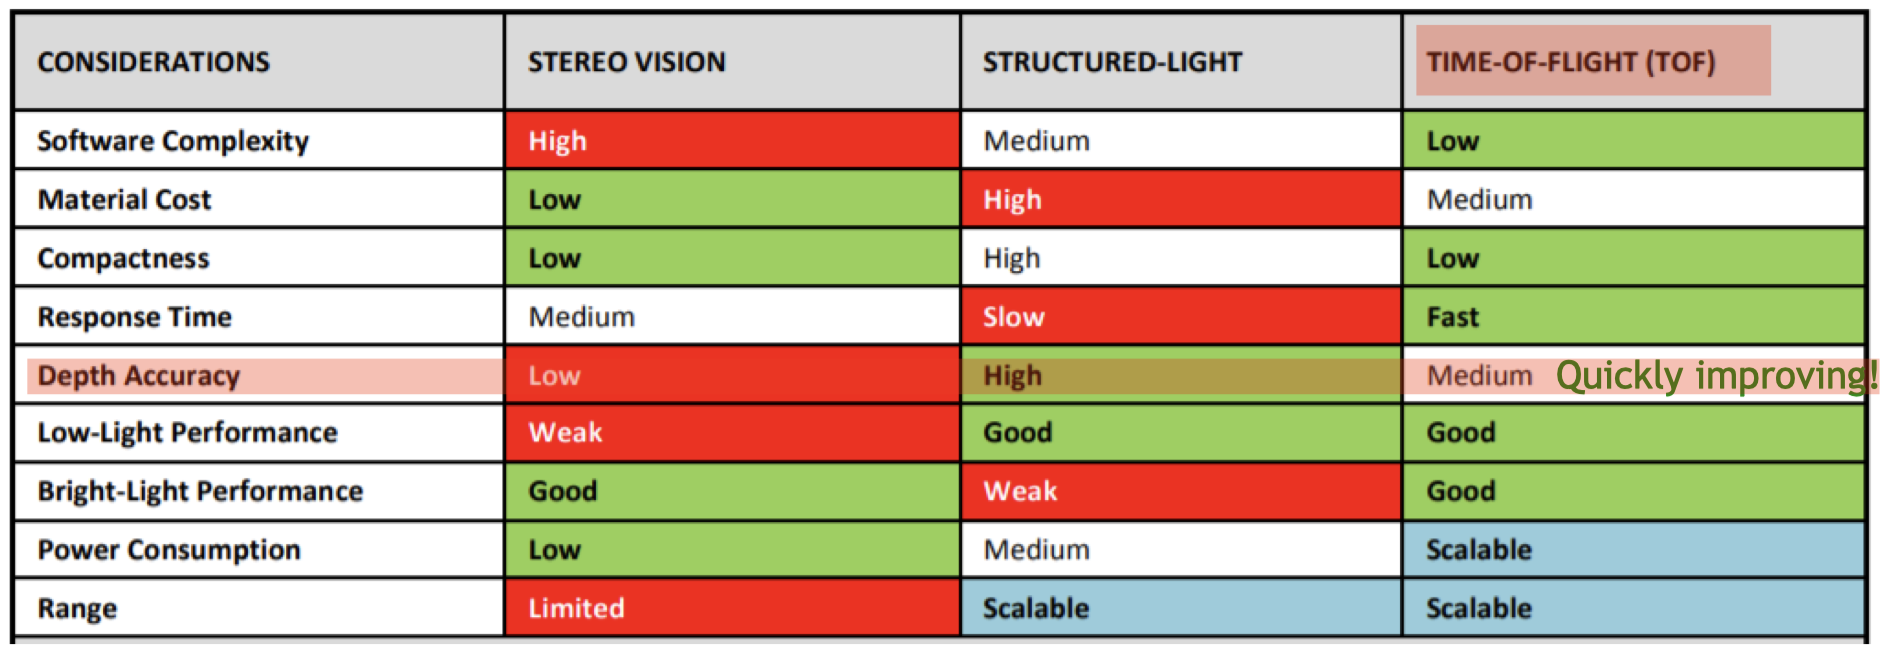
\includegraphics[width=0.7\textwidth]{figures/sensors.png}
    \caption{Summary of Different Depth Sensors}
\end{figure}

\subsection{Multiple 3D representation}

\begin{enumerate}
    \item Multiple images.从各个视角获得的多张图片.它包含3D信息,indirect,not a true 3D representation.
    \item Depth image.只知道深度,不知道相机内参,无法确定两个点的距离.因此被称为2.5D.
    \item Voxels.物体占据了位置则设为1.能被index.但是非常昂贵.$O(n^3)$.没有表面的表示.一旦分辨率低,则无法还原丢失的信息.
    \item Irregular 3D representation. Mesh,point Cloud, Implicit representation.
\end{enumerate}

\subsection{Mesh}

在表面取点,用过三点的平面近似表面.实际上也不限于三角形.下面我们讨论triangle mesh.

\begin{equation}
    \begin{aligned}
        V &= \{v_1, \cdots, v_n\} \in \mathbb R^3
        \\
        E &= \{e_1, \cdots, e_n\} \in V\times V
        \\
        F &= \{f_1, \cdots, f_n\} \in V\times V \times V
    \end{aligned}
\end{equation}


好的mesh:watertight(不漏), manifold(外法向量连续).

\subsection{Point Cloud}

Point cloud是一个$3n$级别的存储方式,当然也可以添加其他分量.它是不规则(irregular)且无序的数据.换言之,其数据的序并不是必要的,
不能提供额外信息,如同set一样.好的算法应该尽可能不去运用序.它是非常轻量级,紧致的,线性级别的存储空间.容易存储,容易理解和生成,容易在其上构建算法.

当然它也不是完美的,比如并不容易通过它判断表面的位置.点云实际上是在表面上采样,那么怎样从一个mesh surface上取样呢?

\textbf{Sampling Strategy:Uniform Sampling.}
计算每个表面的面积,以面积为权独立同分布地选取三角形.在三角形里如何均匀选取呢?仿射变换形成直角三角形,再拼接成矩形.
\footnote{直接拼接成平行四边形如何?对三角形均匀采样可以在正方形 (平行四边形)中采样然后对角线截半.}

但是这样取样之后,在取样量不算非常大的时候,经常会出现不太均匀的情形.此时我们可以采用Farthest Point Sampling(FPS).
目标是选取$N$个点使其两两距离求和最大.但这是一个$\mathcal{NP}$-hard的问题.我们采取一个近似的贪心算法.
我们先均匀选取10000个点.在这10000个点最远的1024个点成为组合优化问题.但仍然比较困难.我们先确定一个点,
最后依次选取最远的点.我们也只是希望点云看起来比较均匀,因此没必要一定取得数学上的最优解.

除此之外,点云的距离度量也成为一个问题,这也是无序带来的问题之一.
我们希望找到一个permutation invariant的度量:Chamfer distance.
\footnote{在某些文献当中,式 \ref{eq:chamfer distance}有时也会带平方.
但是如果带平方,则三角不等式不成立.}

\begin{equation}
    d_{CD} = \sum_{x \in S_1} \min_{y \in S_2} \norm{x - y}_{2} + \sum_{y \in S_2} \min_{x \in S_1} \norm{x - y}_{2}
    \label{eq:chamfer distance}
\end{equation}

对于每个单项,称为uni chamfer distance.在一个点云是另一个子集的时候有用.并且这里似乎应该除以二才能和EMD进行比较.

另一个度量是Earth Mover's distance\footnote{在WGAN中使用.}.与CD不同的是,它要求两个点云数量相同,
且每个点必须找到互不重复的对应.\footnote{Earthmover,中文直译为推土机.
EMD距离用于衡量(在某一特征空间下)两个多维分布之间的dissimilarity,它
的计算基于著名的运输问题.但是精确求解EMD亦非易事,调用的package也多为近似算法.}

\begin{equation}
    d_{E M D}\left(S_{1}, S_{2}\right)=\min _{\phi: S_{1} \rightarrow S_{2}} \sum_{x \in S_{1}} \norm{x-\phi(x)}_{2}
\end{equation}

CD对于取样情况不太敏感,而EMD则比较敏感.比如同样对于Stanford bunny,
如果一个点云多集中在头部,另一个比较均匀,则CD变化不大而EMD变换显著.
由于点云是surface+sampling,因此如果对于取样有要求,应该使用EMD.

\subsection{CD vs EMD}

区别在于 CD 对于采样不敏感,而 EMD 对于采样敏感.

同时EMD需要两个点云点的数量相同.

也就是如果mesh一样但是sample不一样,那么EMD会很大

\subsection{Implicit Representation}

对于一个点,使用一个关于这个点的函数的值来表示这个点是否在物体表面

具体的表示方法是隐式表达,即SDF(signed distance function)

简单地说,这个函数表示空间中点到物体表面的距离,内部为负,外部为正.

其数学定义为:设$\Omega$为度量空间$X$的子集,$d$为$X$的度量,则SDF定义为

\begin{equation}
    f(x)=\begin{cases}
        -d(x, \partial \Omega) & \text { if } x \in \Omega 
        \\
        d(x, \partial \Omega) & \text { if } x \in \Omega^{c}
    \end{cases}
\end{equation}

其中$d(x, \partial \Omega) \xlongequal{\text{def}} \inf_{y \in \partial \Omega} d(x, y)$.

SDF的用处:

\begin{enumerate}
    \item \textbf{collision check:}如果一个东西跟另外一个东西的碰撞。
    那么其中物体A它上面的所有点到底有没有碰到物体B呢?
    我们就可以通过query所有点在B的物体的SDF里头它的值是多少。如果都是大于0,说明A和B没有碰撞
    \item 使用神经网络把物体的几何通过SDF的方式存储下来
\end{enumerate}

\subsubsection{Mesh to SDF}

在处理Mesh到Signed Distance Field (SDF)的转换时,首先需要一些坐标点,
基于这些点的距离值,可以尝试开发算法来计算对应的SDF值

\paragraph{Calculate Unsigned Distance}
在几何处理中,一种基础的方法是计算点到表面的距离 (Unsigned Distance),不区分点是在物体内部还是外部.
这可以通过将所有三角面视为平面,对于每个点,计算其到每个三角面的垂线距离.如果垂足不在三角面上,
则该距离不是最短距离;如果垂足位于三角面上,则从这些距离中找出最短的,即为该点到表面的最短距离.

\paragraph{Unsigned Distance to Signed Distance}
要将Unsigned Distance转换为Signed Distance,使用等高线将空间中的点进行分层表示.
这些等高线描绘了在某些区域距离先减小然后增加,其中距离最近的点附近的区域距离为零,
利用距离为零的区域判断点是在物体的内部还是外部.

\subsubsection{SDF to Mesh}

使用 marching cube

\begin{figure}[H]
    \centering
    \begin{subfigure}
        \centering
        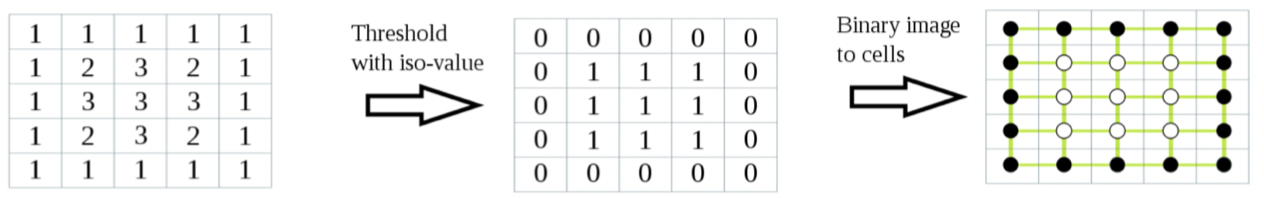
\includegraphics[width=0.7\textwidth]{figures/marching_cube1.png}
    \end{subfigure}
    \vspace{1em} % 调整两个子图之间的垂直间距
    \begin{subfigure}
        \centering
        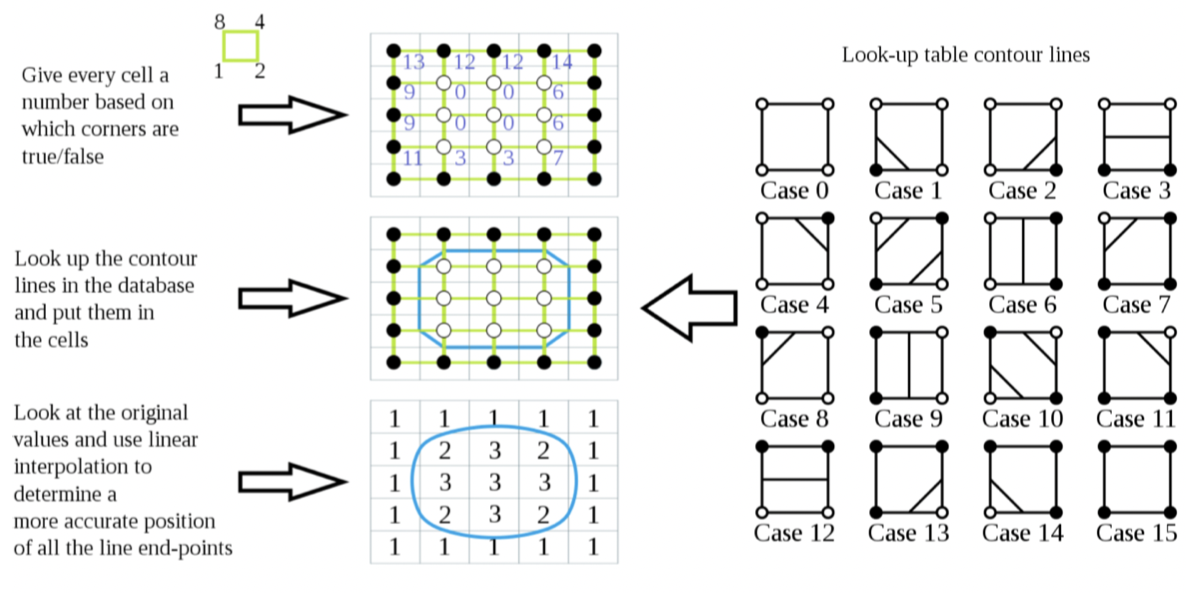
\includegraphics[width=0.7\textwidth]{figures/marching_cube2.png}
    \end{subfigure}
    \caption{Marching cube pipelines}
    \label{fig:marching_cube}
\end{figure}

\begin{enumerate}
    \item 离散化
    \item 二值化
    \item 使用look-up table找轮廓
    \item 使用线性插值优化轮廓
\end{enumerate}

在第三步,很多case都会有这种ambiguity, 如图\ref{fig:mesh reconstruction},所以还需要根据周围的mesh二次优化,决定ambuguity的位置,对于三维mesh重建,这个问题更加严重.

\begin{figure}[H]
    \centering
    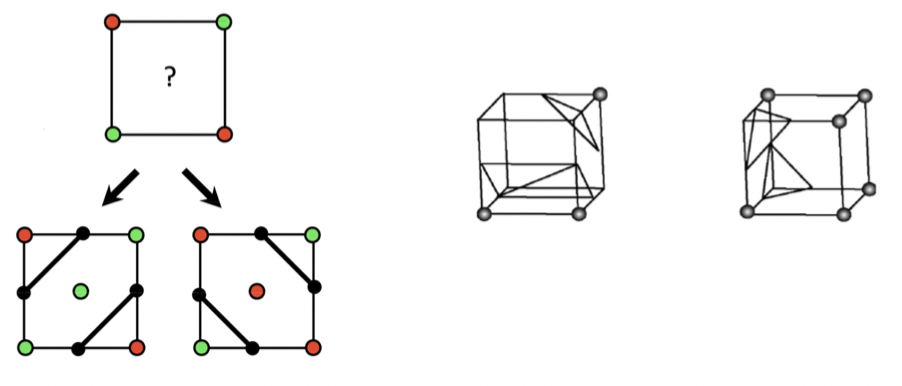
\includegraphics[width=0.7\textwidth]{figures/holes.png}
    \caption{Problem in mesh reconstruction}
    \label{fig:mesh reconstruction}
\end{figure}

\subsection{Deep SDF}

两个trick:

1. 如何分布训练数据点: 如果这个神经网络SDF最终需要使用marching cube,那么应该在SDF为0附近多多采样

2. 训练loss的设置,可以加入一个约束优化:让SDF的梯度为1.这样可以让SDF更加smooth

SDF还满足Eikonel equation,即

\begin{equation}
    \norm{\nabla F} = 1.
\end{equation}

这点不难理解,因为沿与距离最短的点的连线方向的方向导数之模为$1$,而函数本身即表达最短距离, 也就是场变化最快的方向,
不可能沿着梯度前进一个单位的长度,距离变化却超过一单位,因此这也是最大值.

将不同的SDF关联起来,并且保证连续性\cite{Park2019CVPR}

\begin{enumerate}
    \item  use the network to overfit a single shape
    \item use a latent code to represent a shape, so that the
    network can be used for multiple shapes
\end{enumerate}

\subsection{NeRF, 3DGS, Convolution on Mesh/Graph}

了解即可